\subsection{Faltantes}

Para el tratamiento de datos faltantes se indujo valores nulos al 80\% del dataset en los atributos con mayor GainRatio,
se preservó el 20\% de los datos para validación.A continuación se detallan las características de los atributos contemplados:

\definecolor{lightgray}{gray}{0.9}
\begin{table}[H]
\caption{Atributos con mayor GainRatio}
\rowcolors{1}{}{lightgray}
\begin{flushleft}
\begin{tabular}{|>{\centering\arraybackslash}m{5cm}|>{\centering\arraybackslash}m{4cm}|}
\hline
  \rowcolor{blue!55} 
   \multicolumn{1}{|c|}{Atributo} &\multicolumn{1}{c|}{GainRatio} \\ \hline
    inst\_acreditada   &0.0436292021  \\ \hline
    estu\_metodo\_prgm &0.0295357038  \\ \hline
    \end{tabular}
\end{flushleft}
\label{}
\end{table}

El porcentaje de imputación de Missings fue variando de 0 a 0.85 con incrementos de 0.025 generando 36 datasets con datos faltantes. 
En cada generación de Missing ,se relleno con la  moda los datos nulos del atributo inst\_acreditada  y con la modaclase para 
los valores nulos del atributo estu\_metodo\_prgm. Después se construyeron modelos con las estrategias
de relleno de datos faltantes anteriormente descritas variando el CF (Confidence Factor) de 0 a 0.5 y 
finalmente se evaluaron los mismos con el set de validación.

\begin{figure}
  \centering
  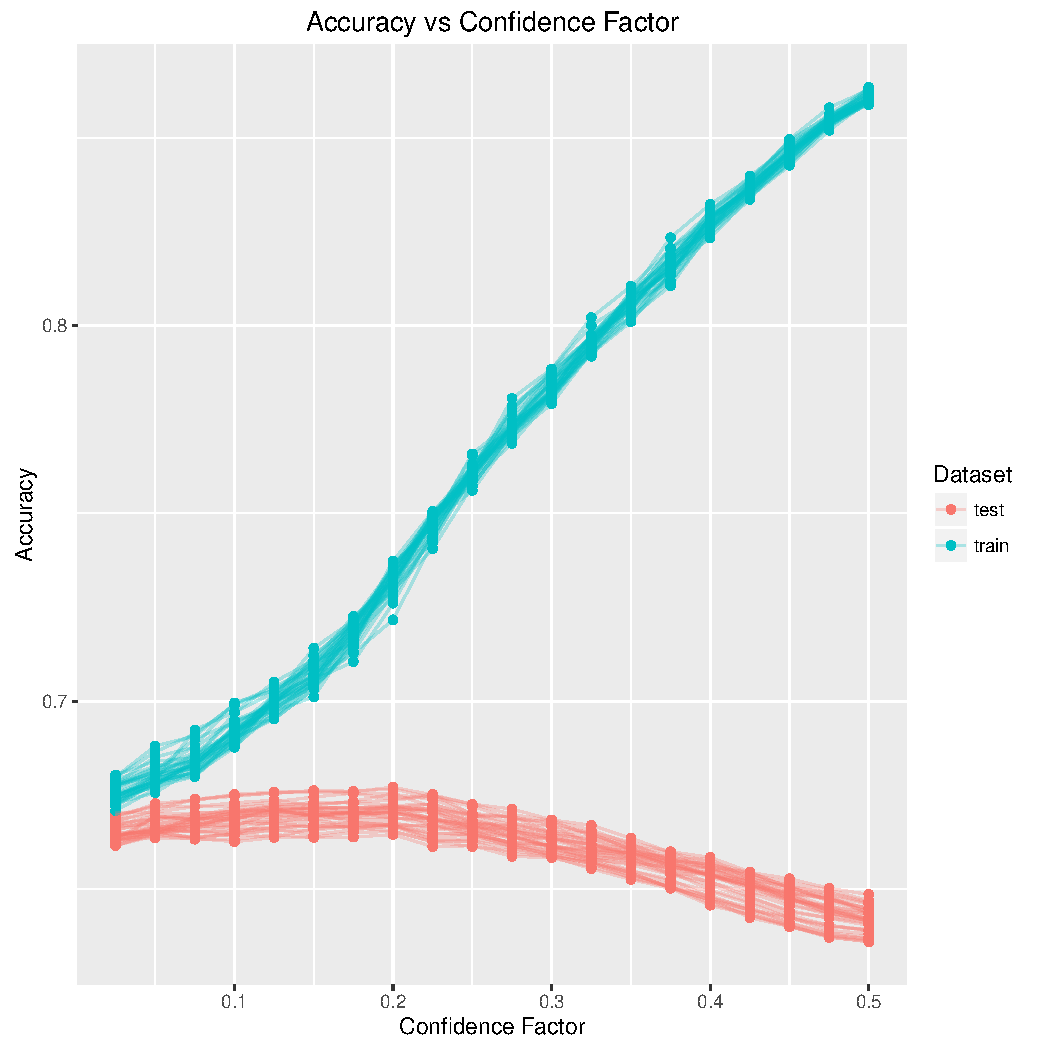
\includegraphics[width = 8cm]{4a.pdf}
  \caption{Accuracy vs Confidence factor with missing data}
  \label{fig:4a}
\end{figure}


En la figura~\ref{fig:4b} Accuracy vs Confidence factor with missing data,

\begin{figure}
  \centering
  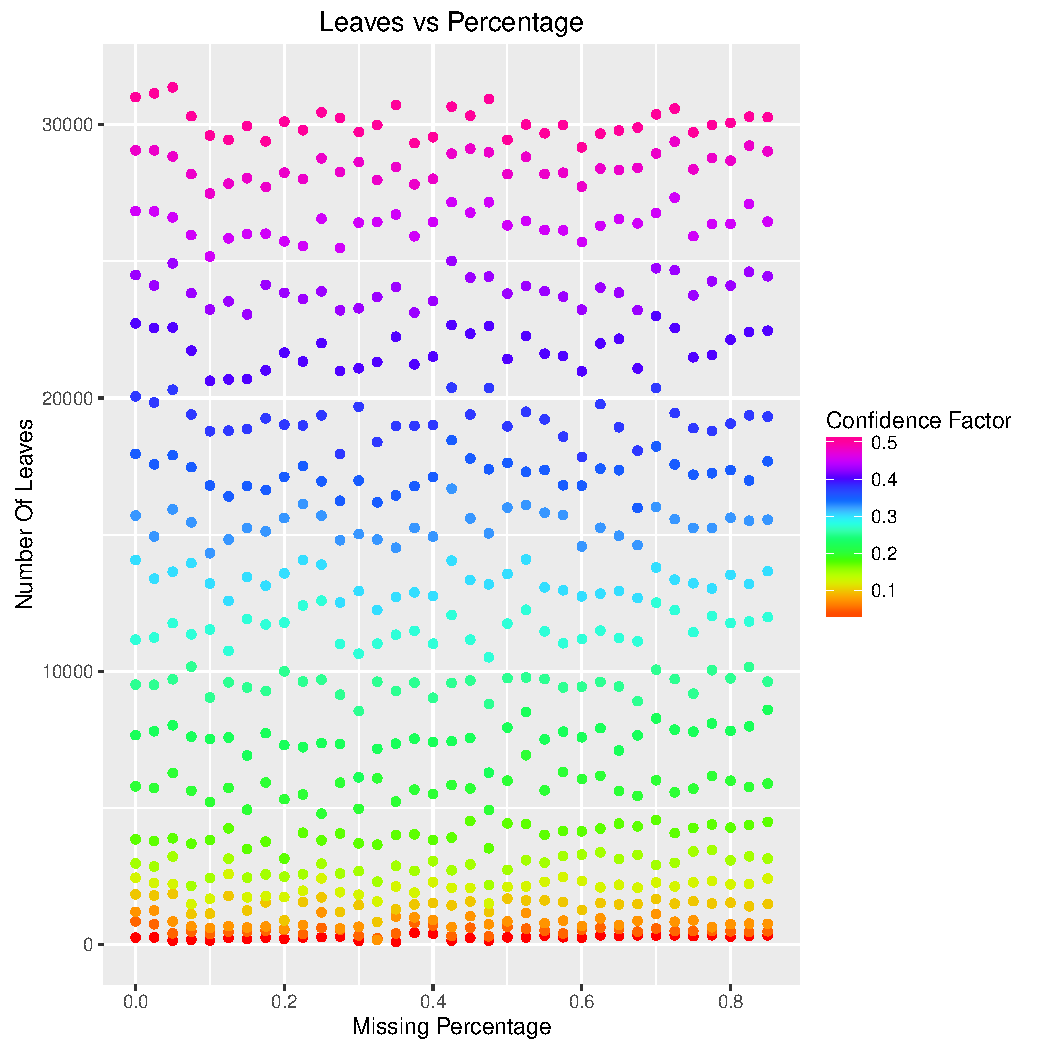
\includegraphics[width = 8cm]{4b.pdf}
  \caption{Leaves vs missing percentage}
  \label{fig:4b}
\end{figure}

En la figura~\ref{fig:4c} Accuracy vs Confidence factor with missing data,

En el gráfico se observa un patrón de comportamiento en las curvas de training y de test para la accuracy
similares a las curvas generadas en las corridas donde no se imputaron datos faltantes,
esto nos dice que el algoritmo J48 presenta resistencia y robustez a datos faltantes independientemente de la función de poda.


\begin{figure}
  \centering
  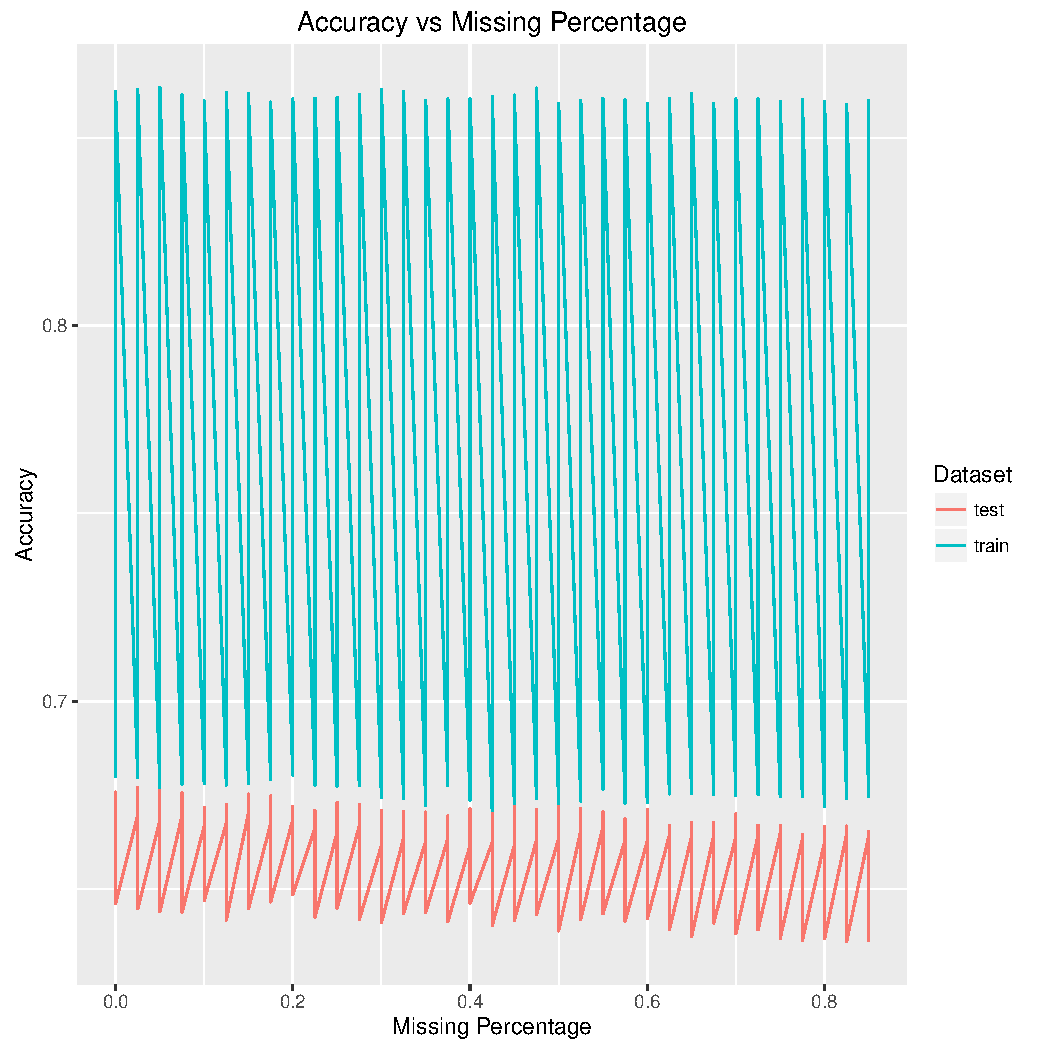
\includegraphics[width = 8cm]{4c.pdf}
  \caption{Accuracy vs missing percentage}
  \label{fig:4c}
\end{figure}

En la figura~\ref{fig:4d} Missing percentage vs Confidence factor,

\begin{figure}
  \centering
  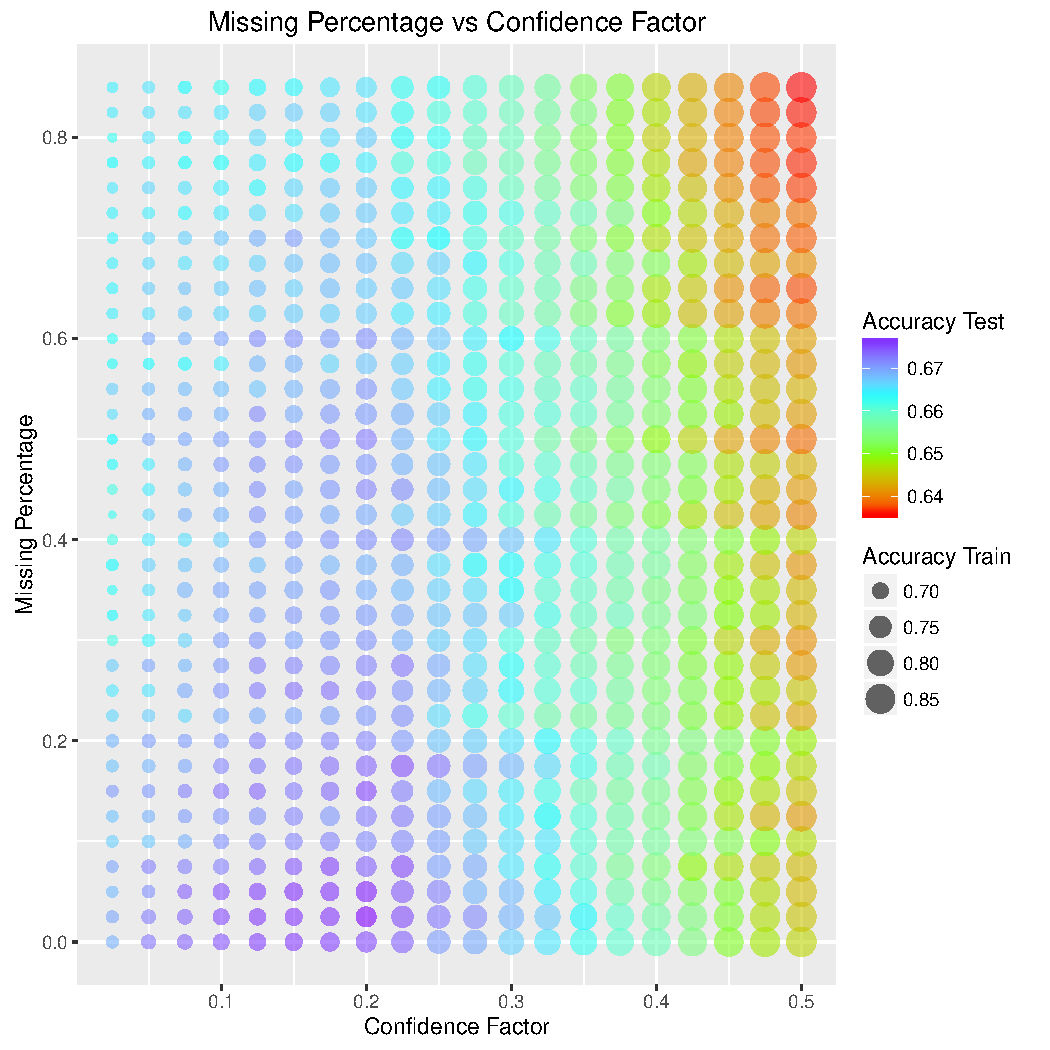
\includegraphics[width = 8cm]{4d.pdf}
  \caption{Missing percentage vs Confidence factor}
  \label{fig:4d}
\end{figure}
